\chapter{Renormalization Group, an Introduction}
\label{ch-renorm-group-intro}

In this chapter, we discuss
the Renormalization Group (RG)
techniques in general.
Other chapters of this book 
on the topic of RG are listed in Section \ref{sec-rg-examples}.

This chapter is based on 
an introduction to RG 
entitled \qt{Honey, I shrunk the theory} that I wrote for some friends in 2011.

\section{Introduction}
 Renormalization Group (RG)
theory
 describes how the observables of
a physical system scale
near a critical point.

The subject of RG theory
includes the following topics:
\begin{itemize}
\item {\bf regularization:}
defining a finite integral
from a  divergent integral.
The parameter in the finite integral
than one takes
the limit of to get the divergent
integral is called the
regulator of the integral.
Divergent integrals arise 
in field theories because such
theories describe an infinite number
of harmonic oscillators, each with
a finite zero point (ground state)  energy.
\item {\bf renormalization:}
a process of possibly
adding a finite number
of new interactions to a field theory
and dividing certain parameters
of the field theory
by normalization constants called $Z_g$
for various  subscripts $g$,
so as to make the
field theory finite. These
normalization constants
are parameterized by a
regulator and diverge as
that regulator tends to a
certain value.
\item {\bf scaling:} a meta-theory
about how a field theory transforms
under scale transformations.
The scaling in RG
is associated with
 the phenomenon of screening,
whereby a charged particle polarizes
its surrounding medium so that
the charge perceived by
an observer (called
the effective charge)
decreases as
the observer moves
away from the particle.



\end{itemize}



RG theory is
truly a big tent.
It has been applied in
a wide variety of scientific disciplines.
Here is a partial list of some of
those areas. 

\begin{itemize}
\item
quantum field theory,
both relativistic (used
in High Energy Physics) and
non-relativistic (used in Condensed Matter
Physics)

\item
statistical mechanics (phase transitions,
Density Matrix Renormalization Group (DMRG))

\item
fluid mechanics (turbulence)
\item
chaos and fractal theory
\item
differential equations

\item
probability and statistics

\item Bayesian Networks, Neural Networks and AI

\item classical Shannon information theory
\item quantum information science, quantum
Shannon information theory,
study of quantum entanglement.
\end{itemize}


There is a huge amount of
literature on RG theory,
and I'm only familiar with
a tiny amount of it.

Two fine books 
by Condensed Matter Physicists on
the sole topic of
RG theory 
  are
Ref.\cite{Mc} by McComb and Ref.\cite{Go} by Goldenfeld.

A fine book by a High Energy Physicist 
that covers RG theory is Ref.\cite{Sr}
by Srednicki. Ref.\cite{Sr}
covers much more than RG theory.
It's a comprehensive  
book on  Quantum Field Theory.


Taste in Physics books is very subjective so
I advise you to inspect the books
I've recommend
and many others too. Then
form your own opinions.

Besides books, I 
found the following 
Wikipedia articles interesting

\begin{itemize}

\item {\bf Renormalization Group},
Ref.\cite{wiki-rg}



\item {\bf Dimensional Analysis},
Ref.\cite{wiki-da}

\item {\bf Landau Pole},
Ref.\cite{wiki-landau-pole}

\item {\bf Scale Invariance},
Ref.\cite{wiki-scale-inv}


\end{itemize}

I've also found asking questions to AI's such as ChatGPT very helpful
as a learning tool.




\section{Scaling and dimensions}



We will use the units 
used in High Energy
Physics in which $\hbar$ (Plank's constant divided by $2\pi$) and $c$ (speed of light) are set to 1 
temporarily, and then restored when one needs actual values in MKS units. In such units,
everything has dimensions of $L^D$, where $L$
stands for length, and $D$ is some rational number. The dimensions of length and time are $L$ and those of energy, mass and
momentum are $L^{-1}$.

Let 

pixel = region between two adjacent lattice sites in 1-dim,
4 adjacent lattice sites in 2-dim, etc.

$x, \ell=$ length in cm (or in any unit of length), a
fixed number of pixels is
contained in one cm

$a=$ lattice spacing, distance between two adjacent pixels.

$b\in[1, \infty]$, length scaling factor, equal to $\ell_i/\ell_f$
where $\ell_i$ (resp. $\ell_f$)
is the length in cm of an initial (resp., final) piece
of the physical system.
(see Chapter \ref{ch-fractal-dim})

$\mu=$ renormalization mass scale, in units
of mass or energy

$\Lam=$ momentum cutoff, in units of momentum

Define (see Fig.\ref{fig-b-funs})
\beq
a(b)= ba_0, \quad
 x(b)= \frac{x_0}{b}
\eeq
\beq
 \Lam(b) = \frac{\Lam_0}{b},
\quad
 \mu(b)=b\mu_0
\eeq
An alternative
notation that is very common is to
use a prime for the output
and to omit the 0 subscript 
for the input. For example, to say
$a'=ba$
and $x'=x/b$ instead of $a=ba_0$
and $x=x_0/b$. 
Alternatively, one could write $a_{i+1}=ba_i$, $x_{i+1}=x_i/b$, etc. for
the steps in an iteration.
At the beginning 
of each iteration (programming loop),
$a_0$ is set equal to $a$,
or $a'$ is set equal to $a$.

Note that $xa$ does not change when
one iterates ($x_0a_0\rarrow xa$). So 
if $a$ goes from $1$ to $2$, 
$x$ is reduced by half.

Note also that
\beq
\ln \mu 
=
\ln \mu_0 +\ln b
\implies \quad d\ln \mu = d\ln b
\eeq

\begin{figure}[h!]
\centering
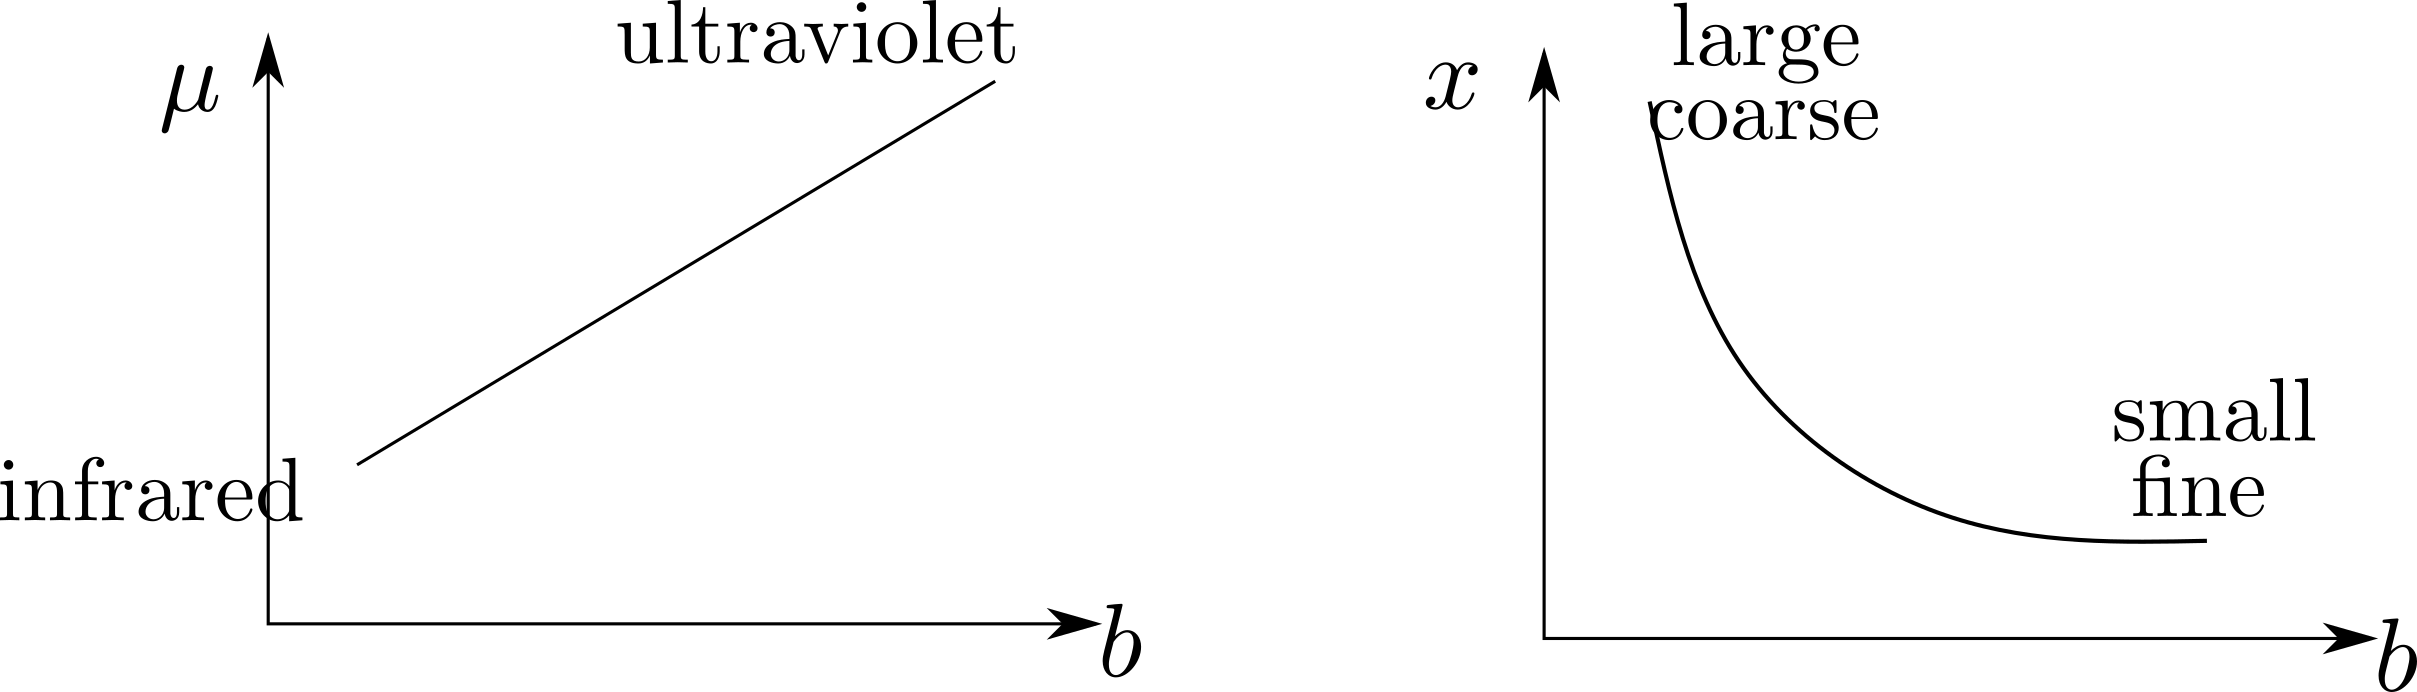
\includegraphics[width=3in]
{renorm-group-intro/b-funs.png}
\caption{Various functions of $b$}
\label{fig-b-funs}
\end{figure}








High Energy Physicists define the {\bf beta
function} for a coupling 
constant $g$ by
\beq
\frac{d g}{d \ln \mu} = \beta(g)
\eeq
Condensed Matter
Physicists define
the {\bf anomalous dimension
or negative fractal dimension}\footnote{For a full
chapter on fractal dimension, see
Chapter \ref{ch-fractal-dim}.
The fractal dimension $D^{frac}$,
the anomalous dimension $y$
and the engineering
dimension $D^{eng}$ are related
by $y=-D^{eng}=-D^{frac}$} $y_q$ of a quantity $q$
by the following equation, valid near a critical point:
\beq
q(b)=b^{y_q}q_0
\label{eq-t-scales-as}
\eeq
For example, 
consider the 2-dim Ising model 
and let $t = \frac{T-T_c}{T_c}$.
Near the  critical point,
Eq.(\ref{eq-t-scales-as})
is satisfied with $q$ replaced by $t$ and $y_t=1$.
Hence, for the 2-dim Ising model, the  temperature deviation grows linearly under coarse-graining.
Thus, the temperature is a relevant operator near the critical point.

Note that

\beq
\ln q =y_q \ln b + \ln q_0
\implies
\frac{d\ln q}{d\ln b} = y_q,\quad\frac{1}{q}\frac{dq}{d\ln \mu}=y_q
\eeq
Hence, 

\beq
gy_g \approx \beta(g)
\eeq

A physical quantity $q$
can be assigdned both an \textbf{engineering dimension} $D_q$
given by dimensional analysis,
and an \textbf{anomalous  dimension}
 $y_q$.
This is expressed by the following 2 equations:

\beq
\engdim{q}=L^{D_q}
\;,
\eeq
and

\beq
q'= b^{y_q} q
\;.
\label{eq-def-fractal}
\eeq
For example,
given 3 quantities $q_j$ for $j=1,2,3$, then

\beq
\engdim{\frac{q_1}{q_2 q_3}}=
L^{D_1-D_2-D_3}
\;,
\eeq
and

\beq
\frac{q'_1}{q'_2 q'_3}
= b^{y_1-y_2-y_3}\frac{q_1}{q_2 q_3}
\;.
\eeq

Note that a length $x$ has
$D_x=1$ and $y_x=-1$\footnote{The fact that $D_x$ and $y_x$
have opposite signs
instead of the same sign,
is a matter of convention. 
Note that mass, momentum and energy
have dimensions of $1/L$. So if we define
$M=1/L$, and the engineering dimension
$D^{eng}$ as $M^{D^{eng}}$ instead of  $L^{D^{eng}}$, then $y=D^{eng}$  instead
of $y=-D^{eng}$.}.
In some cases, it makes sense
to set $y_q=-D_q$ for all quantities $q$.
However, in other
cases, as in the proximity
of a critical point, one cannot set $D_q=-y_q$
for all quantities $q$. 

Let $\phi_x\in \RR$
be the value of a field
at position $x\in \RR^d$. For
each $x$, $\phi_x$ is a dof (degree of freedom) of the
theory. One can also consider
a conjugate dof $\phi_p$
which is the Fourier transform of $\phi_x$.
Only $\phi_p$
for  momenta $p$
in
the ball $\{p: |p|<\Lambda\}$
are allowed.
$\Lambda$,
the maximum momentum magnitude allowed,
 is called the {\bf cutoff
momentum}.


In {\bf real space RG}
applied to a cubic lattice with
lattice constant $a$,
we reduce (lossy data compression) the info in
a $d$-dimensional block with sides of length $x_0$
into the info in a  block with sides of length $x_0/b$.


In {\bf momentum space RG}, we
integrate over the high frequency
dofs in $\{\phi_p:
\Lambda_0/b <|p|<\Lambda_0\}$.
Thus, we reduce the
info in $\{\phi_p: |p|<\Lambda_0\}$
into the info in
$\{\phi_p: |p|<\Lambda_0/b\}$.

In both real and momentum space RG,
we reduce the number of dofs
 of the theory being considered
from $N_{dofs}$ to $N'_{dofs}$, where

\beq
b = \frac{N_{dofs}}{N'_{dofs}}
\;.
\eeq


\begin{tabular}{|
>{\columncolor[HTML]{FFCCC9}}l ||
>{\columncolor[HTML]{CBCEFB}}l |}
\hline
Condensed Matter Physicists: & High Energy Physicists \\ \hline
$b$ & $\mu$ \\ \hline
real space renormalization & momentum space renormalization \\ \hline
coarse graining & integrate over high freq. modes \\ \hline
\end{tabular}

Let $b, b_1,b_2,b_3\geq 1$.
If $R_b$ denotes
a {\bf renormalization transformation (one iteration) 
with scaling factor $b$}, then clearly

\beq
R_{b_1 b_2} = R_{b_1}R_{b_2}
\;.
\eeq
Note that
$R_1 R_b = R_b$
(identity property),
and  $R_{b_1}(R_{b_2}R_{b_3})=
(R_{b_1}R_{b_2})R_{b_3}$
(associative property).
However, one cannot
set $R_{1/b}R_{b}=R_1$ (inverse property)
because $1/b$ is not greater than 1.
Physically,
the reason RG operations
don't have inverses is
that they represent lossy data-compression,
and therefore are irreversible.
So the set of transformation
$\{R_b: b\geq 1\}$
is not a true mathematical
group. In truth, it only
satisfies the properties of
a weaker algebraic
structure called a {\bf semi-group}.\footnote{However,
if the theory is scale invariant (i.e., conformal)
as happens when it sits at a critical point,
then
one can consider all $b> 0$,
not just $b\geq 1$,
and the set $\{R_b: b>0\}$
is a true group.}.
Physicists, however, call it a group
anyway.







\section{Correlations}
\label{sec-corr}

Let
 $\phi_x\in \RR$
be the value of a field
at position $x\in \RR^d$.
 $\phi_x$
is taken to be a random variable.
Let
$\av{Q}$
denote the average of a
quantity $Q$. We will use the
following shorthand notations

\beq
r= |x_1-x_2|,\;\;
\Delta\phi_x = \phi_x - \av{\phi_x}
\eeq
We define the {\bf Greens's function} $G(r)$
by

\beq
G(r) = \av{\phi_{x_1}\phi_{x_2}}
\;,
\eeq
and the \textbf{connected Greens's function}
 $G_c(r)$ by

\beq
G_c(r)=
\av{\Delta\phi_{x_1}\;\;\Delta\phi_{x_2}}
=
\av{\phi_{x_1}\phi_{x_2}}
-\av{\phi_{x_1}}\av{\phi_{x_2}}=
 \av{\phi_{x_1},\phi_{x_2}}
\\
\;.
\eeq
The behavior of $G_c(r)$ near but not precisely
at a critical point is of an
exponential form, with decay
constant given by the {\bf correlation length} $\xi$.
\beq
G_c(r)\sim \exp(-r/\xi)
\eeq



Lossless (resp., lossy) data-compression
of the theory
is associated with zero (resp., non-zero)
$\xi$.
The intuition
for this fact is that a field with
$\xi=0$ is composed of
probabilistically independent dofs $\phi_x$.


As mentioned before, in the
case of lossless (resp., lossy)
data-compression, one can (resp., cannot)
set the engineering and anomalous dimensions
 equal (up to a sign) for every
physical quantity (i.e.,
$y_q=-D_q$ for all $q$).

One can prove that there is
a number $d_{uc}$ called
the \textbf{upper critical dimension},
such that $\xi=0$
if $d\geq d_{uc}$.
For instance, for a $\phi^4$
theory, $d_{uc}=4$. For $d\geq d_{uc}$,
one can \qt{neglect the thermal
fluctuations}, set $\xi=0$,
assume lossless data-compression,
and
set $y_q=-D_q$ for all $q$.
The Landau and mean field
models describe this lossless regime.




\section{RG flows}
A theory is described by a Hamiltonian
$H$. Each interaction term
in the Hamiltonian is
multiplied
by a different \textbf{generalized c.c. (coupling
constant)} $K_j$
which measures
the strength of that
interaction term. 
$\vec{K} = (K_1, K_2, \ldots K_{N_{c.c.}})$
is a point in {\bf c.c. space}.
Applying $R_b$ once
gives

\beq
H' = R_b H,\;\; \vec{K}'=R_b\vec{K}
\;.
\eeq
Applying $R_b$ multiple times gives

\beq
H^{(n+1)}= R_b H^{(n)},
\;\;
\vec{K}^{(n+1)}= R_b \vec{K}^{(n)}
\;,
\eeq

\beq
H^{(n)}= R_b^n H^{(0)},
\;\;
\vec{K}^{(n)}= R_b^n \vec{K}^{(0)}
\;,
\eeq
for $n=0,1,2, \ldots$. The
sequence $\vec{K}^{(0)},
\vec{K}^{(1)}, \vec{K}^{(2)}, \ldots$
specifies 
 a one-dimensional parametric curve in c.c. space
called an {\bf RG streamline or flow}. A different curve
is traced for
each initial condition
$\vec{K}^{(0)}$. The streamlines
flow from $b=1$ to $b=\infty$.

\section{Fixed points}

If, as $n\rarrow \infty$,
\beq
\vec{K}^{(n)}\rightarrow \vec{K}^*
\;,
\eeq
we say $\vec{K}^*$ is a
\textbf{fixed point} in the c.c. space.
Other functions of $\vec{K}$
like the Hamiltonian $H(\vec{K})$
and the correlation length $\xi(\vec{K})$
also tend to a fixed point

\beq
H(\vec{K}^*)=H^*,
\;\;
\xi(\vec{K}^*)=\xi^*
\;.
\eeq


Note that the correlation length
$\xi$ transforms as

\beq
\xi'=\frac{\xi}{b}
\;,\;\;
\xi^{(n)} = \frac{\xi^{(0)}}{b^n}
\;.
\label{eq-xi-zero-to-n}
\eeq
Therefore, for large $n$,
\beq
\xi^* = \frac{\xi^*}{b^n}
\;.
\label{eq-xi-lim}
\eeq
Eq.(\ref{eq-xi-lim}) has two possible solutions.
Either $\xi^* = 0$, in which case
we say the fixed point $\vec{K}^*$
is trivial, or $\xi^* = \infty$,
in which case we say the fixed point
is critical.


\textbf{Trivial fixed points} are not
very interesting. Since they
have $\xi^*=0$, they can be understood
in terms of
lossless data-compression and
engineering dimensions for the c.c.'s.

\textbf{Critical points}
are much more interesting.
Since they
have $\xi^*=\infty$, they can be understood
in terms of
lossy data-compression
and fractal dimensions for the c.c.'s.

The temperature at which
a critical point occurs
is called its {\bf critical temperature}
and is
denoted by $T_c$.
\begin{figure}[h!]
\centering
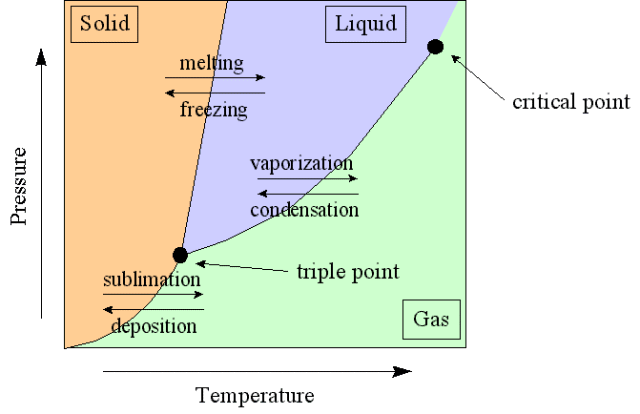
\includegraphics[height=2.5in]
{renorm-group-intro/pd-water.png}
\caption{Phase diagram for water.}
\label{fig-pd-water}
\end{figure}


Two examples of critical points that
occur in Nature are 

\begin{itemize}
\item the Curie temperature of
an Ising system (the temperature
$T_c$ at which the magnetization of a
system at zero
externally applied magnetic field, 
switches between
zero ($T>T_c$) and growing spontaneously ($T<T_c$)).
\item
the critical point of water (a
unique point in the PVT phase diagram
of water, a point at which gaseous and liquid
water coexist). See Fig.\ref{fig-pd-water}.
\end{itemize}



A {\bf first order phase transition (1PT)}
is defined as a locus of points
where the first derivatives of the free
energy are discontinuous. 
A {\bf second order phase transition (2PT)}
is defined as a locus of points
where the first derivatives of the free
energy are continuous but the second derivatives
are  discontinuous.
A critical point and a 2PT are the same thing.


In phase diagram of water in Fig.\ref{fig-pd-water}, 
the 2PT 
(the highest temperature at which liquid and gas phases of water coexist) is the endpoint of a 1PT line.
The triple point of water (a point where
all 3 phases of water coexist)
is not a critical point although
three 1PT lines meet at it.






\section{Relevant operators}

It is interesting
to analyze the behavior
of a field theory in the vicinity
of a critical point.
To do this, it
is convenient to replace
the
generalized c.c.'s
$\vec{K}=(K_1, K_2,\ldots, K_{N_{c.c.}})$
by \textbf{natural c.c.'s}
$\vec{g}=(g_1, g_2,\ldots, g_{N_{c.c.}})$.
The natural c.c.'s are natural
coordinates for describing
the particular
critical point
being considered. They
have the critical point as their origin
(i.e., $\vec{g^*}=0$).

The set of all points that flow into
 the critical point 
is called the \textbf{critical surface or stable manifold
or basin of attraction}.
The set of points that flow away from the critical point is called the {\bf unstable manifold}.
The critical surface is important because it describes all microscopic systems that become critical after coarse-graining.
The unstable manifold describes less 
interesting systems that flee from the critical point.

As a consequence
of Eq.(\ref{eq-xi-zero-to-n}),
all points in the critical surface
have infinite correlation length $\xi$,
just like the critical point
itself.


Note that
\beq
g_j' = b^{y_j} g_j,
\;\;
g_j^{(n+1)} = b^{ny_j} g_j^{(0)}
\;
\eeq
for all $j$. Since $b\geq 1$, there
are three possible scenarios for each
$g_j$:
\begin{itemize}
\item $y_j>1$:
In this case
$g_j^{(n)}\rarrow \infty$
as $n\rarrow \infty$. We say
$g_j$ is a {\bf relevant c.c.}.

\item $y_j<1$:
In this case $g_j^{(n)}\rarrow 0$
as $n\rarrow \infty$. We say
$g_j$ is an {\bf irrelevant c.c.}.
\item $y_j=1$:
In this case $g_j^{(n)}$ tends to a constant
as $n\rarrow \infty$. We say
$g_j$ is a {\bf marginal c.c.}.
\end{itemize}
If an  interaction term in the
Hamiltonian is multiplied by a relevant c.c.,
we call that interaction term a relevant
operator, and likewise for irrelevant and marginal.
For example,
in the 2-dim Ising model (see Chapter \ref{ch-renorm-group-ising}) whose 
Hamiltonian is
\beq
H =
-J\sum_{(i,j)\in\;nn}S_i S_j -
h\sum_{i} S_i
\;,
\eeq
the spin-spin
interaction proportional to 
$J$ is a relevant operator, and the magnetic field 
interaction proportional to $h$ 
is an irrelevant one.


\begin{figure}[h!]
\centering
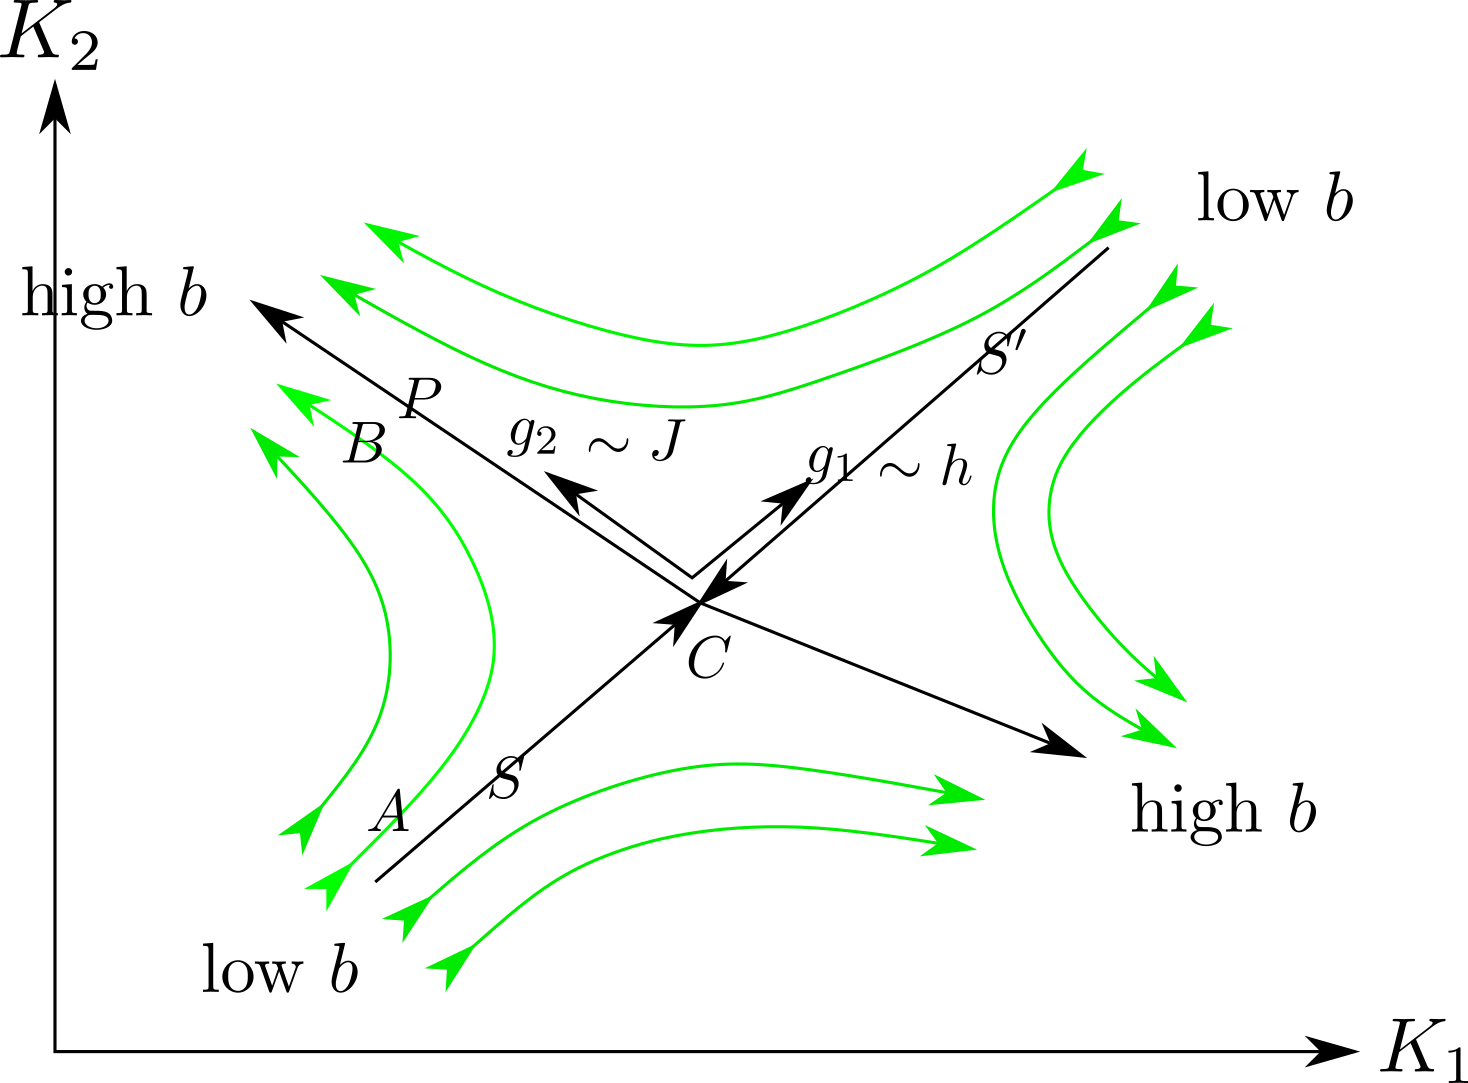
\includegraphics[height=2.7in]
{renorm-group-intro/renorm-group-critical-point.png}
\caption{RG streamlines in
    the vicinity of a critical point
    for a theory with 2 coupling constants.
If one adds a $b$ axis pointing
out of the page, then this
flow diagram 
implies a a 2-dim surface
with a saddle point at $C$.
For a 2-dim Ising model, $g_1$ is $h$ and $g_2$ is $J$.}
\label{fig-rg-critical-point}
\end{figure}



Fig.\ref{fig-rg-critical-point} shows the typical behavior
of the RG streamlines in the vicinity
of a critical point, assuming $N_{c.c.}=2$.
In Fig.\ref{fig-rg-critical-point}, point $C$
is the critical point.
The $K_1,K_2$ axes are for the generalized
c.c.'s and the $g_1, g_2$
axes are for the natural c.c.'s.
The arrows on the streamlines point
in the direction of
increasing $b$.
In the case of Fig.\ref{fig-rg-critical-point},
the {\bf critical surface}
is a
one dimensional curve, the one that contains
points
$S$, $C$ and $S'$.
No streamlines ever cross the
critical surface. For all $b$, the streamlines stay
either above or below the critical surface.

If the initial conditions
are such that the system starts
somewhere on the critical surface,
then for $b$ large enough,
the system ends at point $C$ where
$g_1=g_2=0$. On the
other hand, if the system
starts at a point such as $A$
which is close
to the critical surface but not on it,
then the irrelevant c.c. $g_1$ (resp.,
relevant c.c. $g_2$)
shrinks (resp., grows)
monotonically
as $b$ grows.
By the time the system reaches, say,
point $B$,
$g_1$ is negligible,
and
$g_2$ is starting to become uncomfortably
large for expanding in powers of it.
A good place to do
 perturbation
theory
is in the vicinity of point $P$,
where the irrelevant c.c. $g_1$
is negligible, and the relevant c.c $g_2$
is smaller than 1, but still non-zero.


\section{Critical exponents and universality classes}
How various thermodynamic
quantities behave near and precisely
at a critical point is described
by a slew of
{\bf critical exponents}.
It is common to define
6 critical exponents $\alpha, \beta,
\gamma, \delta,\nu ,\eta$ (all defined
so as to be non-negative). These are
defined on page 150 of McComb.
One
can use very general
thermodynamic arguments to prove
that these 6 exponents must satisfy
4 simple relationships
between them. Thus,
one need only measure 2 of
6. The 2 that are usually measured
are
$\nu$ and $\eta$.

$\nu$ and $\eta$
can both be inferred
from the behavior of the connected Greens's functions $G_c(r)$
defined earlier. Let

\beq
\theta = \frac{\Delta T}{T_c}=
\frac{T-T_c}{T_c}
\;.
\eeq
The behavior of $G_c(r)$ near but not precisely
at a critical point is of an
exponential form, with decay
constant given by the correlation length $\xi$.
The dependance of $\xi$ on temperature
determines the critical exponent $\nu$:

\beq
G_c(r)\sim \exp(-r/\xi),
\;\;
\xi = |\theta|^{-\nu}
\;.
\eeq
(Note that for $\nu>0$,
$\xi\rarrow \infty$ as $T\rarrow T_c$.)
The behavior of $G_c(r)$ precisely at
a critical point is an inverse power
law, and the power of the law
determines the critical exponent $\eta$:


\beq
G_c(r)\sim 1/r^{pow},\;\;pow = d-2+\eta
\;.
\eeq
Let $d=4$. If $\eta=0$, this gives
an inverse square law. If $\eta>0$,
$G_c(r)$ decays faster than
when $\eta=0$,
as one expects if there is screening.

For all
field theories, all critical points
with the same critical exponents
 are
said to be in the same
\textbf{universality class}.
For example, the $\phi^4$ theory
has a single trivial fixed point for $d\geq 4$,
but for $1<d< 4$,
it has a single critical fixed
point, called the Wilson-Fisher (WF) point. The WF fixed point
 has the same critical exponents
as the critical point
of the Ising model in $d$ dimensions.







\section{The regulator and the fiducial
mass scale}
\label{sec-regulator}

A continuous
quantum field
theory has
infinite
terms in its perturbation
expansion. That's
not surprising because
such a theory
describes infinitely many
harmonic
oscillators, and each of
those harmonic oscillators  has a
finite zero-point (ground state) energy of $\hbar\omega/2$.
One regulates the infinities
of a quantum field theory
by introducing a \textbf{regulator}
parameter with a \qt{catastrophic} value.
The
infinities go away if
the regulator is slightly
off from its catastrophic
value, and they come back as
 the regulator
tends to its catastrophic
value.  All
observable
quantities must
be independent of the regulator.
The most popular
regulators used in the RG literature
are
\begin{enumerate}
\item
a momentum cutoff $\Lambda$. 

A  momentum cutoff is used in 
\begin{itemize}
\item Wilson's  integration of UV modes by integrating over 
a shell of momenta $(\Lam/b, \Lam)$, 
\item 
the Pauli-Villars regularization
used in High Energy Physics
to replace propagators $1/(p^2-m^2)$
by $1/(p^2-m^2-\Lam^2)$.
\end{itemize}
\item 
$\epsilon = 4 -d$. 

This is called
dimensional regularization.
It involves analytically continuing
integrals over momentum
to $d\in\RR_{>0}$ dimensions.
In this case, in order to make
the c.c.'s dimensionless,
one needs to introduce a
\textbf{fiducial mass scale}.
This fiducial mass scale,
called
the \textbf{renormalization-point},
is usually denoted by $\mu$.
\footnote{See Chapter \ref{ch-renorm-group-phi-four}
for an explanation
of how the renormalization point
$\mu$ arises in a quantum field theory
from dimensional analysis.}
\end{enumerate}

In case (1), the space-time
dimension $d$ is kept
fixed at an integer value, whereas
in (2), $d$ varies
over a continuum of real
numbers.



In both cases (1) and (2), we use a fiducial mass scale,
$\Lambda$ in case (1) and $\mu$ in case (2).
Roughly speaking,
the fiducial mass scale
parameterizes
how we
subtract the infinite
part of the answer.
In case (1),
$\Lambda$ acts both as
the regulator parameter and
the fiducial mass scale.
In case (2), these
two roles are assigned to
separate parameters, $\epsilon$
becomes the regulator and
$\mu$ the fiducial mass scale.


\section{RG theory pi-groups.
Callan-Symanzik Type Equations}

In doing dimensional
analysis (Ref.\cite{wiki-da})
for a given problem, one
usually begins by finding the
 pi-groups relevant to the
problem. A pi-group (so called
because the symbols $\pi_1, \pi_2, \ldots$
are used to represent them)
is a product
of quantities that is dimensionless:
\beq
\text{
engineering dim of pi-group}=L^0
\;.
\eeq
Analogously, in RG theory, one
can often identify certain compound
quantities which must be scale
invariant (i.e., independent
of $\mu$).
I like to call such
quantities RG pi-groups.

\beq
\frac{d}{d\ln \mu}
\{\mbox{\rm RG pi-group}\}=0
\;.
\label{eq-callan}
\eeq
The Callan-Symanzik equation
used in High Energy Physics is
just a special case of Eq.(\ref{eq-callan}).


\section{Examples of use of RG theory}
\label{sec-rg-examples}

This book describes how to 
apply RG theory to 3 physical systems:

\begin{enumerate}
\item RG for Ising Model, Chapter \ref{ch-renorm-group-ising}

\item RG for $\phi^4$ theory, Chapter \ref{ch-renorm-group-phi-four}

\item RG for Bayesian Networks, Chapters \ref{ch-ising-dbnet}
and \ref{ch-renorm-group-bnets}
\end{enumerate}


